% =============================================================================
% Report for the Solar Filament Segmentation Challenge 2026 (Kaggle).
% Based on the organizers' Overleaf template (acmart, sigconf). Template packages
% live in preamble.tex; citations live in main.bib.
% =============================================================================

\documentclass[sigconf]{acmart}
% =============================================================================
% Template setup — participants normally do not edit this file.
% Author content belongs in main.tex; citations belong in main.bib.
% \documentclass lives in main.tex so Overleaf does not treat this file as root.
% =============================================================================

% --- Competition / non-ACM-submission friendly rights metadata -------------
\setcopyright{none}
\settopmatter{printacmref=false}
\acmConference[Kaggle Competition]{Filament Segmentation Challenge}{2026}{\href{https://www.kaggle.com/competitions/filament-segmentation-2026}{kaggle.com/competitions/filament-segmentation-2026}}
\acmBooktitle{Competition Report}
\acmDOI{}
\acmISBN{}

% --- Author guidance text --------------------------------------------------
% \guide{...} is gray italic while \guideStyletrue; omitted from the PDF if false.
% Flip the switch in main.tex after % =============================================================================
% Template setup — participants normally do not edit this file.
% Author content belongs in main.tex; citations belong in main.bib.
% \documentclass lives in main.tex so Overleaf does not treat this file as root.
% =============================================================================

% --- Competition / non-ACM-submission friendly rights metadata -------------
\setcopyright{none}
\settopmatter{printacmref=false}
\acmConference[Kaggle Competition]{Filament Segmentation Challenge}{2026}{\href{https://www.kaggle.com/competitions/filament-segmentation-2026}{kaggle.com/competitions/filament-segmentation-2026}}
\acmBooktitle{Competition Report}
\acmDOI{}
\acmISBN{}

% --- Author guidance text --------------------------------------------------
% \guide{...} is gray italic while \guideStyletrue; omitted from the PDF if false.
% Flip the switch in main.tex after % =============================================================================
% Template setup — participants normally do not edit this file.
% Author content belongs in main.tex; citations belong in main.bib.
% \documentclass lives in main.tex so Overleaf does not treat this file as root.
% =============================================================================

% --- Competition / non-ACM-submission friendly rights metadata -------------
\setcopyright{none}
\settopmatter{printacmref=false}
\acmConference[Kaggle Competition]{Filament Segmentation Challenge}{2026}{\href{https://www.kaggle.com/competitions/filament-segmentation-2026}{kaggle.com/competitions/filament-segmentation-2026}}
\acmBooktitle{Competition Report}
\acmDOI{}
\acmISBN{}

% --- Author guidance text --------------------------------------------------
% \guide{...} is gray italic while \guideStyletrue; omitted from the PDF if false.
% Flip the switch in main.tex after \input{preamble}.
%
% Do not use \guide{...} for \email{...}.
\usepackage{xcolor}
\newif\ifguideStyle
\guideStyletrue
\newcommand{\guide}[1]{%
\ifguideStyle
{\color{gray!65}\itshape #1}%
\fi
}

% --- Math ------------------------------------------------------------------
% Do NOT load amssymb (or amsfonts): acmart already loads newtxmath, which
% defines the same symbols (e.g. \Bbbk) and causes a conflict on Overleaf.
% amsmath is already provided by acmart; mathtools extends it.
\usepackage{mathtools}

% --- Figures ---------------------------------------------------------------
% graphicx is already loaded by acmart
\usepackage{subcaption}

% --- Tables ----------------------------------------------------------------
% booktabs is already loaded by acmart
\usepackage{tabularx}
\usepackage{multirow}

% --- Bibliography style is set in main.tex (ACM-Reference-Format) ----------
.
%
% Do not use \guide{...} for \email{...}.
\usepackage{xcolor}
\newif\ifguideStyle
\guideStyletrue
\newcommand{\guide}[1]{%
\ifguideStyle
{\color{gray!65}\itshape #1}%
\fi
}

% --- Math ------------------------------------------------------------------
% Do NOT load amssymb (or amsfonts): acmart already loads newtxmath, which
% defines the same symbols (e.g. \Bbbk) and causes a conflict on Overleaf.
% amsmath is already provided by acmart; mathtools extends it.
\usepackage{mathtools}

% --- Figures ---------------------------------------------------------------
% graphicx is already loaded by acmart
\usepackage{subcaption}

% --- Tables ----------------------------------------------------------------
% booktabs is already loaded by acmart
\usepackage{tabularx}
\usepackage{multirow}

% --- Bibliography style is set in main.tex (ACM-Reference-Format) ----------
.
%
% Do not use \guide{...} for \email{...}.
\usepackage{xcolor}
\newif\ifguideStyle
\guideStyletrue
\newcommand{\guide}[1]{%
\ifguideStyle
{\color{gray!65}\itshape #1}%
\fi
}

% --- Math ------------------------------------------------------------------
% Do NOT load amssymb (or amsfonts): acmart already loads newtxmath, which
% defines the same symbols (e.g. \Bbbk) and causes a conflict on Overleaf.
% amsmath is already provided by acmart; mathtools extends it.
\usepackage{mathtools}

% --- Figures ---------------------------------------------------------------
% graphicx is already loaded by acmart
\usepackage{subcaption}

% --- Tables ----------------------------------------------------------------
% booktabs is already loaded by acmart
\usepackage{tabularx}
\usepackage{multirow}

% --- Bibliography style is set in main.tex (ACM-Reference-Format) ----------


% Guide styling: \guideStyletrue = show gray italic hints; \guideStylefalse = omit them
\guideStylefalse

\newcommand{\TBD}[1]{\textbf{\color{red}[TBD: #1]}}

\begin{document}

\title[Consensus U-Nets, PQ-Optimal Selection and Instance Refinement]{Consensus-Supervised U-Nets with PQ-Optimal Instance Selection and Refinement for Solar Filament Segmentation}
\subtitle{A Solution to the Solar Filament Segmentation Challenge 2026} % DO NOT CHANGE

\author{Tatu Helander}
\affiliation{%
\institution{Cloudforge Oy}
\city{Tampere}
\country{Finland}
}
\email{tatu.helander@gmail.com}

% final numbers (scripts/make_decision_table.py, Kaggle)
\newcommand{\pqfinal}{0.448}
\newcommand{\lbfinal}{0.39}

\begin{abstract}
This report describes our solution to the Solar Filament Segmentation Challenge~2026, a Kaggle competition on automatic segmentation of solar filaments in GONG H-$\alpha$ observations. Ten U-Nets (EfficientNetV2-S and EfficientNet-B3 encoders, five date-grouped folds each) are trained at native resolution with \emph{soft consensus} targets, the fraction of annotators who marked each pixel. Their averaged probability map is converted into instances in two learned stages. A decision layer, adapted from a public competition notebook, thresholds the map at 16 levels, scores every nested connected component with a gradient-boosted model of its expected matched IoU against a random annotator, and selects the pixel-disjoint subset that maximises the competition's pooled Panoptic Quality (PQ) with an exact dynamic programme. A second U-Net then re-segments every selected instance from a local window. On all 707 training images the out-of-fold pooled PQ rises from 0.405 (threshold and minimum area) to \pqfinal, with a gain on every fold, and the public leaderboard score from 0.35 to \lbfinal; two annotators scored against each other reach 0.34. Code, trained weights and a notebook reproducing the submission are public.\footnote{\url{https://github.com/cloudforge-oy/solar-filament-2026}}
\end{abstract}

\maketitle

% ==================================== %
% INTRODUCTION %
% ==================================== %
\section{Introduction}
This report goes over the details of our submitted solution to the Solar Filament Segmentation Challenge~2026 \cite{filament-segmentation-2026}. The challenge, launched on July~10,~2026, is organized by the Earth-Space AI Research (ESAIR) Lab\footnote{\href{https://www.esairlab.com/home}{www.esairlab.com/}}. This challenge utilizes the MAGFiLO dataset for evaluation of the segmentation algorithms \cite{ahmadzadeh2024dataset}.

The task is \emph{instance} segmentation evaluated with Panoptic Quality \cite{kirillov2019panoptic}: every predicted filament counts either as a true positive (IoU~$>0.5$ with a ground-truth filament) or as a false positive, and each pixel may belong to at most one prediction. Three properties of the data shaped our design. First, the 707 training images carry 1154 annotation sets, because 296 images were annotated independently by two or three annotators, and the annotators disagree strongly: scoring one annotator's outlines against another's on these images gives a pooled PQ of only 0.340 (mean matched IoU 0.63, recognition quality 0.54). Second, filaments are small and thin (median area 1228~px in a 2048$\times$2048 frame), so down-sampling destroys the barbs the organizers care about. Third, only 0.9\% of the 8199 annotated filaments touch another filament within 3~px, so the problem is almost entirely semantic segmentation followed by a decision about \emph{which} connected regions to submit and \emph{how far} each extends. We therefore pair semantic U-Nets \cite{ronneberger2015unet} with two learned, metric-driven stages, and measure every design choice on out-of-fold data.

% ==================================== %
% METHODOLOGY %
% ==================================== %
\section{Methodology}\label{sec:methodology}

\begin{figure*}[t]
\centering
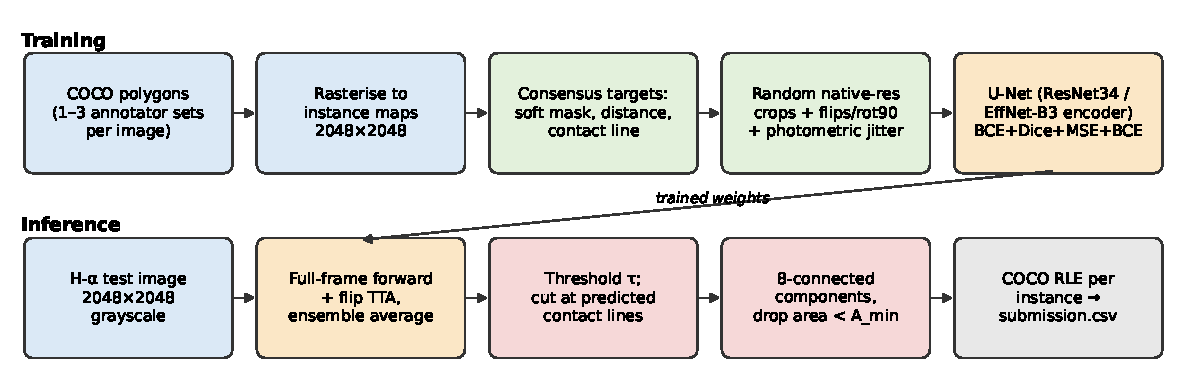
\includegraphics[width=\textwidth]{figures/pipeline.pdf}
\caption{End-to-end pipeline. Training (top): COCO polygons of all annotator sets are rasterised into instance maps and reduced to three consensus targets per image; U-Nets are trained on random native-resolution crops. Inference (bottom): full-frame prediction averaged over eight dihedral views and ten models, a 16-level component tree, a learned score per candidate with an exact selection that maximises pooled PQ, instance-wise refinement, COCO RLE encoding.}
\label{fig:pipeline}
\end{figure*}

\subsection{Data preparation and targets}
Images are read as single-channel 8-bit grayscale; no limb-darkening correction or disk masking is applied. For every annotation set the polygons are rasterised with \texttt{pycocotools}, which reproduces the \texttt{area} field of the annotation file exactly and is therefore the rasteriser behind the hidden ground truth (integer \texttt{fillPoly} rasterisation overlaps these masks with a mean IoU of only 0.87). The $k$ annotation sets of an image are reduced to three \emph{consensus} targets: (i) the soft filament mask $y_{\mathrm{seg}}\in[0,1]$, the fraction of annotators who marked the pixel, so that the network predicts the \emph{expected} annotation; (ii) a normalised distance-to-boundary map, averaged over annotators; (iii) a contact-line map of pixels within 2~px of two instances of one annotation set. The two auxiliary targets were meant to separate touching filaments; neither a distance-map watershed \cite{beucher1993watershed} nor a contact-line cut ever improved validation PQ, so they are kept as auxiliary tasks whose predicted maps serve as candidate descriptors (Section~\ref{sec:decision}).

\subsection{Dense models and training}
We use the U-Net of \texttt{segmentation\_models\_pytorch} \cite{iakubovskii2019smp} with ImageNet-pretrained encoders, one input channel and three output channels, trained with
$\mathcal{L}=\mathrm{BCE}+\mathrm{Dice}$ on the soft mask, $5\,\mathrm{MSE}$ on the distance map and $0.5\,\mathrm{BCE}_{w=20}$ on the contact map. Two encoder families are averaged: EfficientNet-B3 \cite{tan2019efficientnet} (640-px crops, batch 6, 50 epochs, inputs standardised with dataset constants) and EfficientNetV2-S \cite{tan2021efficientnetv2} (512-px crops, batch 16, 75 epochs, inputs standardised with each image's own mean and deviation inside the solar disk). Crops are taken at native resolution, four per image per epoch, centred near a filament pixel with probability 0.7; augmentations are flips, 90$^\circ$ rotations, gamma, contrast, brightness and noise. Optimisation uses AdamW (weight decay $10^{-4}$), a one-cycle schedule peaking at $3\cdot10^{-4}$ and mixed precision; one fold takes 45--50 minutes on an RTX~4080.

\paragraph{Validation split.} The 707 images are grouped by observation date and the dates are assigned to five folds, so that the same day observed by two GONG stations, or the same image annotated by three annotators, never straddles the training/validation boundary. Every model is trained once per held-out fold, so each of the 1154 annotation sets receives an out-of-fold prediction; the two later stages are fitted on these out-of-fold maps with the same folds (\emph{cross-fitting}), and all numbers in Section~\ref{sec:evaluation} are out-of-fold end to end.

\subsection{PQ-optimal instance selection}\label{sec:decision}
Each image is processed as a whole 2048$\times$2048 frame; predictions are averaged over the eight views of the dihedral group (flips and 90$^\circ$ rotations) and over the models. The conversion of this map $p$ into instances follows the decision layer of a public competition notebook \cite{tushhaaarrrr2026filseg}, re-implemented on our own maps (\texttt{src/decision.py}). The host pools TP, FP, FN and matched IoUs over all (image, annotator record) pairs, so
\[
\mathrm{PQ}(P)=\frac{\sum_i R_i\sum_{c\in P_i}u_i(c)}{\tfrac12\sum_i R_i|P_i|+\tfrac12 N_G},\quad u_i(c)=\frac1{R_i}\sum_{r}\mathrm{IoU}(c,g_r)\,\mathbf 1\{\mathrm{IoU}>0.5\},
\]
with $R_i$ the number of records of image $i$ and $u$ the \emph{annotator-expected matched IoU} of candidate $c$. By Dinkelbach's theorem \cite{dinkelbach1967fractional} the optimal submission maximises $\sum_c(u(c)-\tau)$ with one global $\tau=\mathrm{PQ}^*/2$.
\textbf{Candidates.} $p$ is thresholded at 16 levels ($0.05,\dots,0.80$); each mask is closed (5$\times$5 ellipse) and hole-filled. Both operations are increasing, so the 8-connected components of all levels ($\geq$100~px) form an exactly nested forest ($\approx$176 nodes per image) whose antichains are exactly the valid pixel-disjoint submissions.
\textbf{Scorer.} 69 descriptors per node feed gradient-boosted trees \cite{friedman2001gbm}: $\hat h$, the probability that a record matches the node, trained on (node, record) rows, and $\hat m$, the expected IoU given a match; $\hat u=\hat h\,\hat m$. Besides level, shape, statistics of $p$ and of the auxiliary maps, darkness against the background, position and station, the descriptors describe the node's \emph{place in its tree} (how many levels it survives, how it splits, its ancestors and siblings, its rank among the image's candidates), its neighbourhood, and the mean probability of each encoder family. Four scorers with different seeds, each split seeing a random half of the descriptors, are averaged.
\textbf{Selection.} $\max\sum_{c\in A}(\hat u(c)-\tau)$ over antichains $A$ is solved exactly by $\mathrm{best}(v)=\max\{0,\hat u(v)-\tau,\sum_{w\in\mathrm{ch}(v)}\mathrm{best}(w)\}$. $\tau$ is the centre of the out-of-fold plateau (Figure~\ref{fig:sweep}). The scorer is fitted on out-of-fold maps of one model per family, while test maps average five; they are smoother and the scorer then keeps fewer instances at the same $\tau$. At test time $\tau$ is therefore set, without labels, to the value that restores the cross-validated number of instances per image (6.9).

\subsection{Instance refinement}\label{sec:refine}
$p$ estimates the probability that a \emph{random} annotator marks a pixel. For a filament that only some annotators draw, $p$ is low everywhere inside it and no level set gives the outline an annotator would draw. The second stage (\texttt{src/refine.py}) is a UNet++ \cite{zhou2018unetpp} with a ResNet34 encoder \cite{he2016resnet} that sees a native-resolution window around \emph{one} selected instance (four channels: image, $p$, the instance, the other selected instances) and predicts $q(x)$, the probability that $x$ lies inside the annotator's outline given that the annotator drew this filament. Its target is the mean of the ground-truth outlines matched to the seed (IoU~$>0.5$). Training seeds are the out-of-fold selections and near-selections of the decision layer ($\approx$86 per image, drawn 12\,000 per epoch for ten epochs on 256-px windows); the refiner of fold $k$ never sees fold-$k$ images. At inference the window is the instance's bounding box plus 48~px, $q$ is averaged over four flips and the five fold models, and the refined mask is the part of $\{q>0.45\}$ connected to the seed. It may not enter another selected instance, instances take pixels in descending score order, and a refined mask whose area leaves $[0.4,3]$ times the seed area falls back to the seed, so the submission stays pixel-disjoint.

% ==================================== %
% EVALUATION %
% ==================================== %
\section{Evaluation}\label{sec:evaluation}

\subsection{Strategy}
We re-implemented PQ as defined by the organizers: predicted and ground-truth instances are matched by IoU~$>0.5$ against every annotation set of an image, and TP, FP, FN and matched IoUs are \emph{pooled} over all 1154 (image, record) pairs as the host does. Every number below is out-of-fold for the dense models, the scorer and the refiner at once.

\subsection{Results}
Table~\ref{tab:ladder} lists the steps in the order they were added, and Table~\ref{tab:decision} the final pipeline per fold. The plain rule (components of $p>0.6$ with area $\geq400$) and the best single tree level score the same (0.405 and 0.407), so the gain of the decision layer does not come from the closing or the extra levels: it keeps fewer, better candidates (false positives fall from 4153 to 2686 for 12 fewer true positives on the final maps). Tree-context descriptors are the most useful addition to the scorer ($+0.006$); geometry, neighbourhood and scorer hyper-parameters each change PQ by less than 0.002. A second encoder family raises the ceiling of the candidate trees (selection with the true $u$: 0.559 to 0.568) but the realised score by only 0.001. The refiner adds $+0.006$ and improves every fold. Trained on an earlier selection, UNet++ scored 0.449, a plain U-Net 0.446 and their average 0.448, so refiner variants differ by no more than run-to-run variation.

\begin{table}[h]
\caption{Pooled out-of-fold PQ (707 images) and public leaderboard score as components were added. Rows without a leaderboard entry were not submitted on their own.}
\label{tab:ladder}
\centering\small
\begin{tabular}{lcc}
\toprule
Pipeline & OOF PQ & public LB \\
\midrule
EfficientNet-B3, flip TTA, plain rule & 0.405 & 0.35 \\
+ decision layer (35 descriptors) & 0.431 & 0.37 \\
+ 8-view TTA, tree-context descriptors & 0.439 & 0.38 \\
+ averaged scorers & 0.441 & -- \\
+ EfficientNetV2-S family & 0.442 & -- \\
+ instance refiner (final) & \textbf{\pqfinal} & \textbf{\lbfinal} \\
\bottomrule
\end{tabular}
\end{table}

\begin{table}[h]
\caption{Final pipeline per fold, pooled out-of-fold PQ: plain rule, decision layer, decision layer with refiner, and the selection with the true $u$ (ceiling of the candidate trees without refinement).}
\label{tab:decision}
\centering\small
\begin{tabular}{lccccc}
\toprule
Fold & plain rule & decision layer & + refiner & $\Delta$ & oracle $u$ \\
\midrule
0 & 0.415 & 0.441 & \textbf{0.450} & +0.035 & 0.569 \\
1 & 0.390 & 0.436 & \textbf{0.444} & +0.054 & 0.563 \\
2 & 0.422 & 0.451 & \textbf{0.459} & +0.037 & 0.575 \\
3 & 0.400 & 0.433 & \textbf{0.442} & +0.042 & 0.566 \\
4 & 0.401 & 0.438 & \textbf{0.442} & +0.042 & 0.571 \\
\midrule
all & 0.405 & 0.440 & \textbf{0.447} & +0.042 & 0.568 \\
\bottomrule
\end{tabular}

\end{table}

\begin{figure}[h]
\centering

\includegraphics[width=\columnwidth]{figures/sweep.pdf}
\caption{Pooled out-of-fold PQ of the decision layer against the selection threshold $\tau$ (cross-fitted scorer), with the plain rule and the best single tree level. The vertical line marks the centre of the plateau.}
\label{fig:sweep}
\end{figure}

\paragraph{What did not help.} (i) Averaging more dense models beyond the two families. (ii) Letting a candidate group fragments at a low threshold while keeping the tighter shape of a high one: the oracle ceiling does not move (0.558 on fold~0). (iii) A CNN that scores each candidate from its image window, used as extra descriptors: trained with early stopping it adds $+0.0004\pm0.0015$; trained to near-zero training loss it adds $+0.003$, but only on images within three days of a training image, i.e.\ by memorising how the same filament was labelled on a neighbouring day. We left it out.

\begin{figure*}[t]
\centering
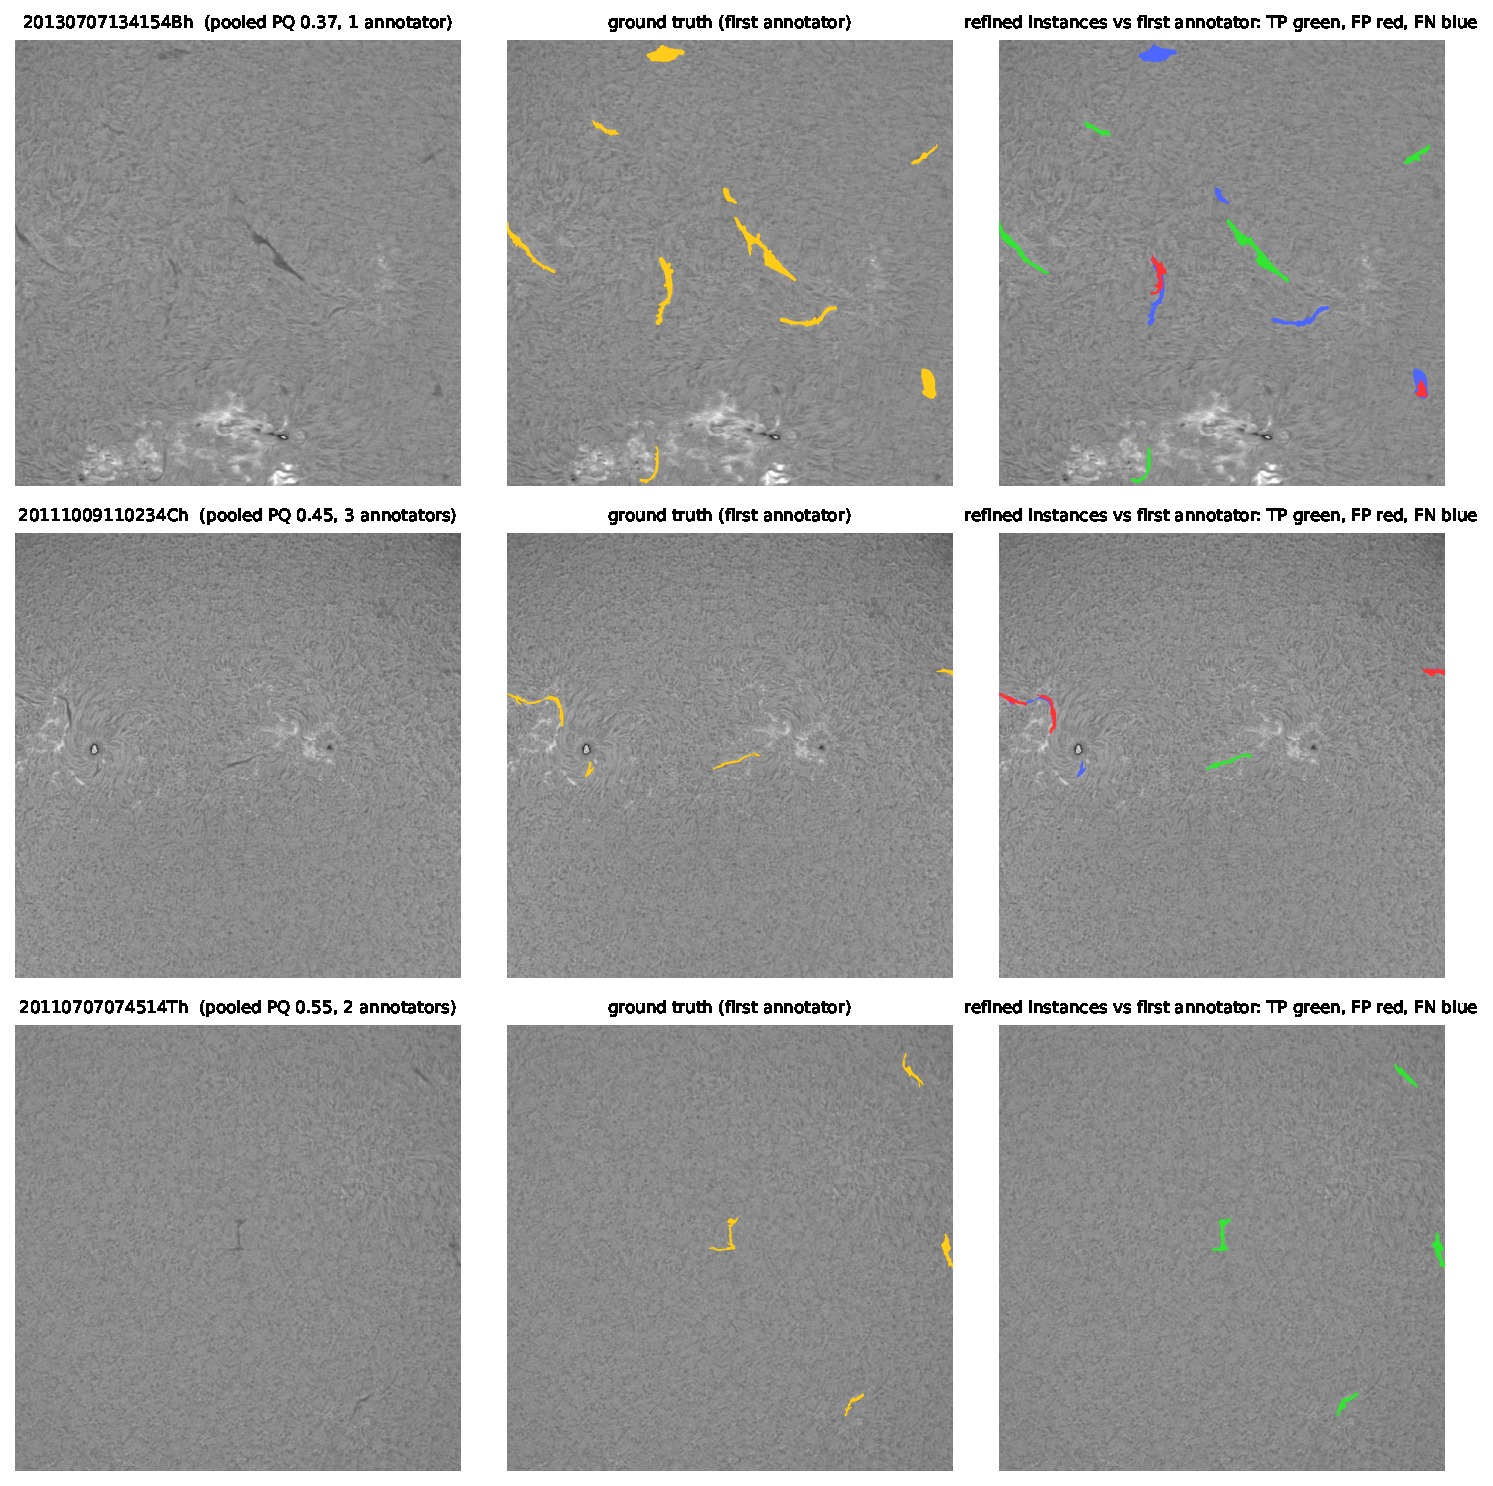
\includegraphics[height=0.40\textheight]{figures/examples.pdf}
\caption{Fold-0 validation images at the 25th, 50th and 75th percentile of per-image pooled PQ (out-of-fold maps, scorer and refiner). Left: H-$\alpha$ crop; middle: the first annotator's ground truth; right: refined instances coloured against that annotator (true positive green, false positive red, missed filament blue). In the top row the pipeline submits as one instance what this annotator drew as two filaments, so neither is matched.}
\label{fig:examples}
\end{figure*}

\subsection{Discussion}
\paragraph{Strengths.} Every stage optimises the competition metric directly and is validated without leakage across folds; the submission is pixel-disjoint by construction; inference takes about 17~s per image on a laptop GPU.

\paragraph{Limits.} The score is bounded by annotator disagreement rather than by image evidence: our out-of-fold PQ (\pqfinal) is already well above the agreement between two annotators (0.340), and with the true $u$ the candidate trees would reach 0.57, so most of the remaining loss is in guessing which faint filaments a particular annotator draws and how they group fragments. Every honest pipeline we could inspect, including ours, loses $\approx$0.06 between out-of-fold and public leaderboard PQ, for models of very different strength, which points to the labels of the public test images rather than to overfitting. Public leaderboard scores above 0.5 should be read with care: the published scorer counts every prediction that overlaps a ground-truth filament by IoU~$>0.5$, so repeating a mask adds true positives \cite{perseus2026flaw}; applied to our own out-of-fold predictions, duplication alone would move 0.44 to 0.52--0.66. All our submissions are pixel-disjoint, as the rules require.

\paragraph{Possible improvements.} Modelling annotator styles, and letting the selection score the refined rather than the raw mask.

% ==================================== %
% ACKNOWLEDGMENT %
% ==================================== %
\section{Acknowledgment}
The organization of the Filament Segmentation Challenge 2026 is partially supported by the U.S. National Science Foundation (NSF) under Grant No. 2209912 and 2433781, directorate for Computer and Information Science and Engineering (CSE), and Office of Advanced Cyberinfrastructure (OAC), and Grant No. 2511630, AST Division Of Astronomical Sciences and MPS Directorate for Mathematical and Physical Sciences.

The Filament Segmentation Challenge 2026 is sponsored by the U.S. National Science Foundation (NSF) National Solar Observatory (NSO).

This work utilizes GONG data obtained by the NSO Integrated Synoptic Program, managed by the National Solar Observatory, which is operated by the Association of Universities for Research in Astronomy (AURA), Inc. under a cooperative agreement with the National Science Foundation and with contribution from the National Oceanic and Atmospheric Administration. The GONG network of instruments is hosted by the Big Bear Solar Observatory, High Altitude Observatory, Learmonth Solar Observatory, Udaipur Solar Observatory, Instituto de Astrofísica de Canarias, and Cerro Tololo Interamerican Observatory.

\bibliographystyle{ACM-Reference-Format}
\bibliography{main}

\end{document}
